\documentclass[letterpaper,onecolumn,titlepage]{Ythesis}
\usepackage[utf8]{inputenc}
\usepackage{tikz}
\usepackage{array,multirow}
\usepackage{subcaption}
\usepackage{subfiles}
\usepackage{url}
\usepackage{amsmath}
\usepackage{float}
\usepackage{graphicx}
\usepackage[backend=bibtex, style=numeric-comp]{biblatex}
\bibliography{glasslab_viz}



\title{Make any stupid plot you want}
\author{Hannah Aizenman}
\committee{Dr. Michael Grossberg (Advisor), Dr. Robert Haralick, Dr. Lev Manovich, Dr. Huy Vo}
\submitted{}
\abstract{}
\begin{document}
\makefrontmatter

\section{Introduction}
\label{sec:introduction}
\begin{figure}
    \includegraphics[width=.5\textwidth]{figures/intro/dubois_bookplate}
    \caption{This collection of visualizations is the inside cover art of W. E. B. Du Bois's Data Portraits\cite{duboiscenterattheuniversityofmassachusettsBoisDataPortraits2018}}
    \label{fig:dubois_bookplate}
\end{figure}

Why am I starting with DuBois? 

 Some of DuBois visualizations are common chart types most modern visualization tools (cite excel, tableu, matplotlib, ggplot, maybe high chart) support, while others are far more custom and likely need tools with drawing capabilities (cite: matplotlib, base r, d3) \cite{duboiscenterattheuniversityofmassachusettsBoisDataPortraits2018}. This intentionality in what charts the tool supports and the flexibility it gives the user underpins why we care about this problem. Drawing programs don't really have to care about the data structure because everything is explicit - the user chooses the shape, line, color, they are by hand manually doing all the encoding. Visualization libraries on the other hand allow users to specify which bits of the data they want encoded and how, but there's a lot of implicit mapping of the raw variables in the data to the encodings. We want some confidence that the visualization tool is making the mapping we intended. We often do this by implictely encoding the data structure in the grammar of the visualiztion tool (grammaer of graphics, vega, ggplot, altair), but a goal of Matplotlib \cite{huntermatplotlib2007} is to be fairly data structure agnostic. We are proposing an architecture that converts these implicit assumptions into explicit contracts between the data and the visualization. 

 Why functional?
 because what we care about is the interface, the contract between the data and the visualization. We need the minimal amount of information that fulfills our contract that we can then put on the screen. (insert react notes here). Our theoretical framework is that that visualization is a transformation from one topological space to another to a CW complex (this probably needs to be explained more), and a functional programming paradigm allows us to directly express that in code. 

 \subsection{What will be the work}
 %%this comes from the grant
 Matplotlib needs to support use cases across a vast range of science domains, enabling complex visualizations [1]. At the same time, common visualizations in a domain need to be fluid for the end-practitioners, tuned to the domain's standard data structures, and with domain-specific customization options exposed. To achieve both of these goals, we need to continue to foster a two-layer ecosystem with a shared core (Matplotlib) and many domain-specific libraries (seaborn, nipy, ...).

In the current grant cycle we have been developing a new architecture that is heavily invested in cleanly separating the three steps in a visualization pipeline: data representation, encoding the data as visual elements, and rendering those elements to screen. We believe that a better delineation of these steps will allow domain practitioners to more easily implement extensions. Following on the work done this year to design consistent data and artist abstractions, we will develop simpler and more expressive user-level APIs in core Matplotlib and in collaboration with domain-specific libraries. 



 Why topology?

 The difference between a line plot and a scatter plot is the former assumes that the data is continous, the latter that it is discrete (cite line and scatter - friendly?) In concrete implementation terms, matplotlib's imshow assumes that the data is continous and therefore does implementation, the matshow assumes it is discrete so it does not. And there are visualization types like area charts that allow even more information to be encoded bewteen the lines. When redesigning the architecture, we needed a way to articulate the differences between the different plot types and found that a topological approach allowed us to encode connectivity (discrete versus continous), dimensionality (point, line, area), and how much information the visualization encodes. 

 What even is data?
 Remake this graph notated w/ graph semantics:
 \begin{figure}
    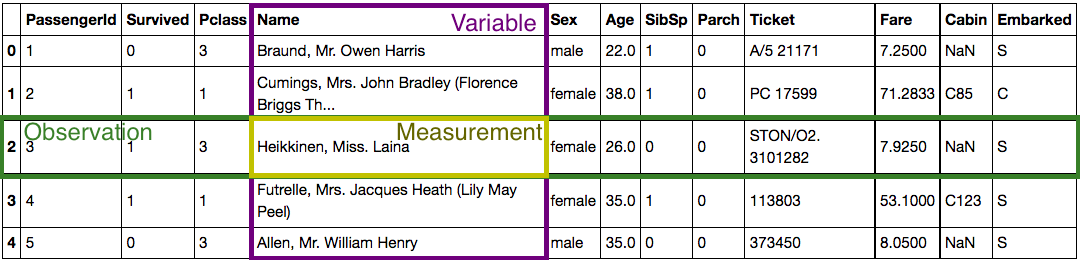
\includegraphics{figures/intro/data_formatting}
    \caption{Modified from Munzner's Visualizarion Analysis and Design}
 \end{figure}

 What even is encoding?

 \begin{figure}
    %% Bertin's decomposition of an image
 \end{figure}
 \begin{figure}
    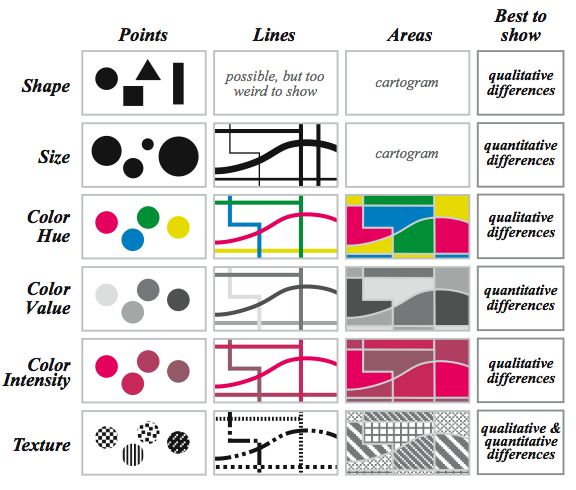
\includegraphics{figures/intro/retinal_variables}
    \label{fig:retinal_variable}
    \caption{This organization of Bertin's retinal variables \cite{bertinSemiologyGraphicsDiagrams2011} that lays out the geometry(marks) and corresponding aesthetic variations (channels) with a recommendation based on data type (qualitative versus quantative) comes from Krygier and Wood's Making Maps \cite{krygierMakingMapsVisual2005}}
\end{figure}

When talking about encodings, we are referring to Bertin's codification of the properties of the graphic system \cite{bertinIIPropertiesGraphic2011} seen in fig~\ref{fig:retinal_variable} as visual variables. In this system, there are the marks, which are the point, line, and area geometric primatives on the visual plane that each represent a single instance of the data being visualized \cite{bertinIIPropertiesGraphic2011,munznerMarksChannels2014}. These marks can be varied along different visual channels  size, value, texture, color, orientation, shape, and position \cite{bertinIIPropertiesGraphic2011, munznerMarksChannels2014}. As shown in fig~\ref{fig:retinal_variable}, the marks encode topological connectivity such that they have the following graph semantics:

\begin{description} 
    \item[Points] - 0d, no edges
    \item[Lines] - 1d, every vertex has <=2 edges (1d simplex)
    \item[Area] - 2d,  every vertex has <=4 edges (2d simplex)
\end{description}

The visual channels in fig~\ref{fig:retinal_variable} are recommended based on the measurement type, quantative versus qualitativem  and Munzner generalizes the quantative channels as magnitude channels for ordered attributes (measurements drawn from an ordered set of possible values) and the qualitative channels as identity channels for categorical attributes (random set of possible values). 


\begin{figure}
    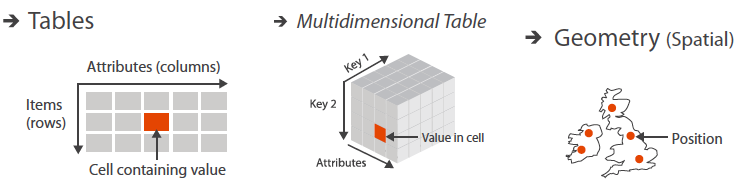
\includegraphics{figures/intro/munzner_datatypes}
    \label{fig:munzner_datatypes}
    \caption{Keys are unique lookup values used to find individual observations in the dataset. Keys are positional references, and can be coordinates on a map or unique values such as a primary key in a database or a (time, latitude, longitude) index in a data cube. Image modified from a diagram from Munzner's website\cite{munznerChDataAbstraction}}
\end{figure}
Munzner's key/value semantics\cite{munznerWhatDataAbstraction2014}
provide a way to identify variables that in effect act as metadata for other variables, such as how when we are interested in the temperature at a time the temperature is the lookup value. But that did not generalize well for complex heterogenous datasets. In this proposal, we refine those ideas by using topology to formally describe the connectivity between the measurements. 

\begin{verbatim}
make any stupid plot you want in robust & rigourous way
        * need rich description langauge + right choice of paradigm (functional) 
        * ability to mathemetaically formalize/conceptual framework for doing this
        * data -> artist, need to preserved the structure of the data moreso than the data 
            * how points are connected to each other
    * targeted implementation rather than protocal (numpy)
        * visualization libraries bound to the datastructures (concrete implementation)
            * encode a lot of assumptions about data in the data structure
            * MPL assume x/y plotted in order you want them in 
            * topology makes the assumptions explicit
            * explicit->math->functional  
    * spell out the layers of visualization libaries:
        * Data + computation -> visualization composites -> drawing library
        * domain specific library
        * utility library <- formalize this piece (SciPy Diagram)
    * viz - Munzner + Bertin
    * functional programming makes sense 
\end{verbatim}


\section{Library Review}
\subsection{Grammar of Graphics \& ggplot}
\begin{figure}
    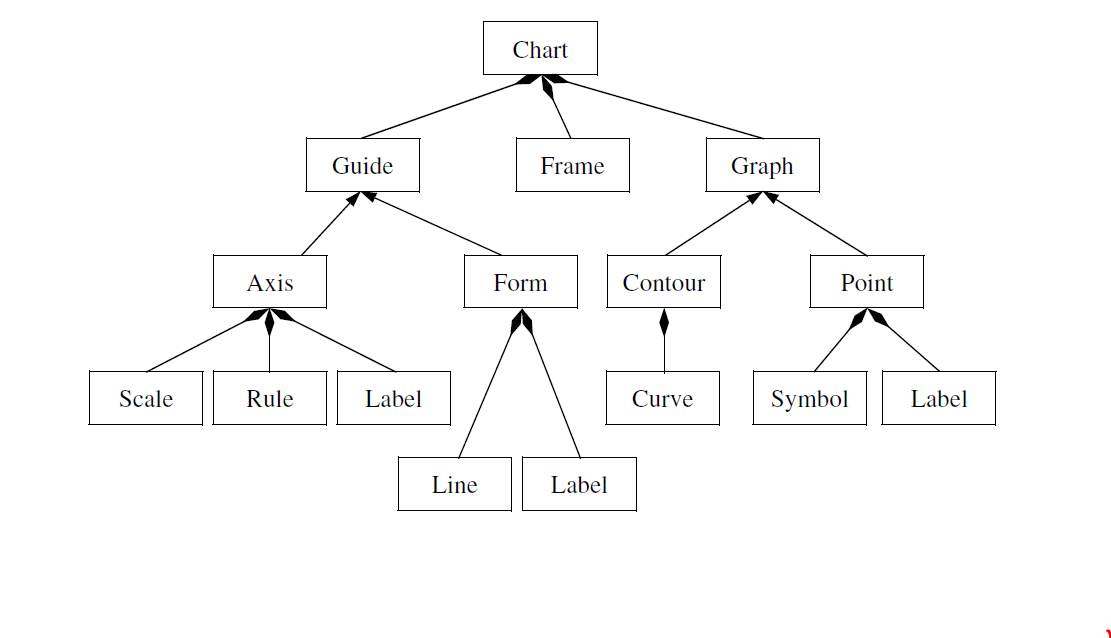
\includegraphics{figures/intro/grammar_chart_composition.png}
    \caption{page 10 (introduction)}
\end{figure}
\begin{figure}
    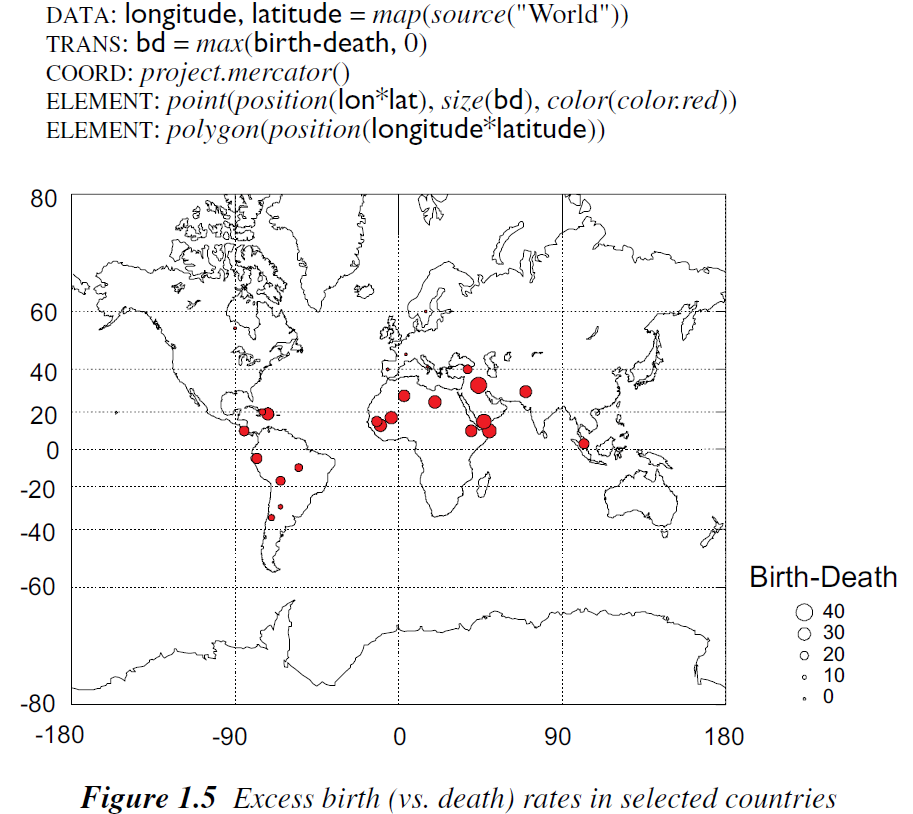
\includegraphics{figures/intro/grammar_example.png}
    \caption{Wilkenson decomposed a graphic into ...} 
\end{figure}
\cite{wilkinsonGrammarGraphicsStatistics2005}
charts - words 
    - instances of much more general objects (geometric primatives)
    - histogram =/= bar chart
graphics - statements 
expliceltly OO
    1. specification
        data - operations/computations
        trans - variable transforms (rank)
        scale - scale transforms
        coord - coordinate system
        element - marks and channels
        guide - meta elements - (axes, legends, etc)
    2. assembly - kinda what happens in artist (spec->something that can go to renderer) 
    3. display - rendering

How is our proposal different? seperation in spec between what's data, aesthetics, and render specific, and what part of the architecture owns those operations





\cite{wickhamGgplot2ElegantGraphics2016}


\printbibliography
\end{document}